\documentclass[tikz,border=2pt]{standalone}
\usepackage{amsmath}
\usetikzlibrary{arrows.meta}
\begin{document}
% APV of a survival payment: 100 paid at time 5 only if T_x > 5 is discounted by v^5 = (1.04)^{-5}
% and weighted by the survival probability 0.9, giving 100(1.04)^{-5}(0.9) = 73.97 at time 0.
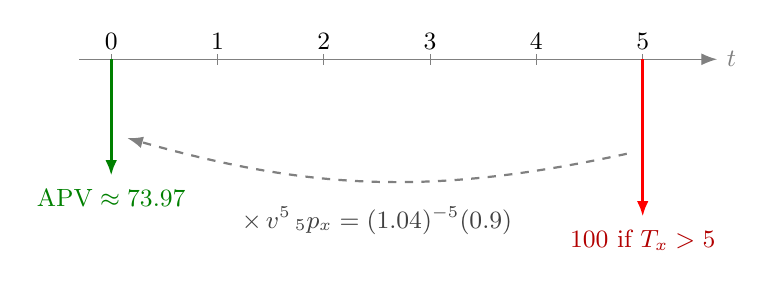
\begin{tikzpicture}[font=\small, >={Latex[length=2mm]}, x=1.35cm, y=1cm]
  \draw[gray, ->] (-0.3,0) -- (5.7,0) node[right] {$t$};
  \foreach \k in {0,...,5} {
    \draw[gray] (\k,-0.07) -- (\k,0.07);
    \node[above, inner sep=2pt] at (\k,0.05) {$\k$};
  }
  % payment at time 5, conditional on survival
  \draw[->, red, very thick] (5,0) -- (5,-2.0);
  \node[red!70!black, anchor=north] at (5,-2.05) {$100$ if $T_x>5$};
  % its actuarial present value at time 0
  \draw[->, green!50!black, very thick] (0,0) -- (0,-1.48);
  \node[green!50!black, anchor=north] at (0,-1.53) {$\operatorname{APV}\approx73.97$};
  % discounting and survival weighting
  \draw[->, gray, thick, dashed] (4.85,-1.2) to[bend left=14] (0.15,-1.0);
  \node[gray!50!black, anchor=north] at (2.5,-1.75) {$\times\,v^5\,{}_5p_x=(1.04)^{-5}(0.9)$};
\end{tikzpicture}
\end{document}
